\chapter[Visualization of the epileptogenic zone on brain images]{Visualization of the epileptogenic zone on brain images}

\chaptermark{Visualization of the epileptogenic zone on brain images}
\label{chap:svt}

\minitoc


\begin{center}
  \begin{minipage}[b]{0.9\linewidth}
    \small
    \textbf{Foreword\,}
    This chapter describes the software developed in the context of a collaboration with neurologists Ali Alim-Marvasti and Gloria Romagnoli.

    My contributions to this project are:
    \begin{itemize}
      \item A 3D Slicer module \cite{fedorov_3d_2012} that reads the output of the querying tool and generates a 3D visualization on a parcellated brain \ac{MRI}, where the brightness associated to each brain structure is proportional to the probability of the \ac{EZ} being in the structure.
      \item The software engineering aspects of the project: a \ac{PIP}-installable Python package for the querying tool, including \ac{CI}, and an \ac{API} to access the Python package from 3D Slicer or from the command line.
      \item The implementation of the online demo, which does not require installing 3D Slicer%
      \fnurl{https://github.com/fepegar/SVT-web}.
    \end{itemize}
  \end{minipage}

  \begin{minipage}[b]{0.9\linewidth}
    \small
    Ali and Gloria performed the systematic literature review to generate the database (which is an Excel spreadsheet) that maps seizure semiologies to brain regions.
    Ali wrote most of the code to query the database, and contributed to the Slicer module.
    The code and the database are available on GitHub%
    \fnurl{\svtgithub}.

    The relevant publications are:
    \begin{itemize}
      \item \bibentry{perez-garcia_towards_2020}
      \item \bibentry{perez-garcia_towards_2020-1}
      \item \bibentry{alim-marvasti_probabilistic_2021}
      \item \bibentry{alim-marvasti_mapping_2021}
    \end{itemize}

  \end{minipage}
\end{center}

\acresetall
\bodyspacing
\section{Introduction}

\Acp{ASM} is normally used to treat epilepsy.
One third of epilepsies are drug-resistant \cite{engel_what_2016}.
Curative resective surgery can be performed to remove the \ac{EZ} (\cref{chap:resection}).
The location of the \ac{EZ}, ``the area of cortex indispensable for the generation of clinical seizures'' \cite{rosenow_presurgical_2001}, is normally inferred by a multidisciplanary team following non-invasive evaluation such as video-\ac{EEG}, \ac{MRI} or neuropsychological tests.
If the information regarding the location of the \ac{EZ} is clear and concordant between the different tests, curative resection may be performed to treat the epilepsy.
Otherwise, \ac{iEEG} electrodes may be implanted to localize the \ac{EZ} precisely.
% To determine the brain regions that may be involved in the \ac{EZ} which need to be recorded to resolve the \ac{EZ}, i.e., the targets for the \ac{iEEG} electrodes, the team leverages information from the non-invasive examinations, including seizure semiology from the recorded videos (\cref{chap:videos}).  % Rachel
To determine the brain regions that need to be implanted with electrodes, the team leverages information from the non-invasive examinations, including seizure semiology history from patients and witnesses, and from the recorded videos (\cref{chap:videos}).  % John
% To determine the brain regions that need to be recorded, i.e., the targets for the \ac{iEEG} electrodes, the team leverages information from the non-invasive examinations, including seizure semiology from the recorded videos (\cref{chap:videos}).  % original
The choice of targets is therefore influenced by the team's subjective experience and personal knowledge of the literature.
This leads to substantial variations of implantation strategies across different epilepsy centers \cite{tufenkjian_seizure_2012}.
The diagnostic pathway for surgical planning could be supported and standardized by an objective tool to aid clinicians in deducing the \ac{EZ} location from seizure semiology.

% Rachel's suggestion to replace the paragraph above
It would be useful for clinicians to be able to quickly and easily assess relevant studies in the literature for a specific semiology.
Such a method has been proposed \cite{alim-marvasti_probabilistic_2021} using a database of studies analyzed via the \ac{PRISMA} framework.
Clinicians and researchers would benefit from a easy-to-use and intuitive \ac{GUI} to such a database.
Moreover, visualizing the probability of each structure containing the \ac{EZ} on \ac{3DMMI} could help plan either resection or \ac{iEEG} implantation strategies \cite{nowell_resection_2017, nowell_utility_2015}, potentially using \ac{ATP} \cite{sparks_automated_2017}.
Finally, a \ac{3DMMI} visualization could be used to perform qualitative and quantitative analyses of the retrospective information contained in the \svtdatabase database.

In this work, we present a software tool that, given an observed list of seizure semiologies and other patient data such as the dominant hemisphere, generates a table with the number of datapoints associated to each brain region.
% Each datapoint represents a patient presenting the observed semiologies who became seizure-free after resection of the corresponding brain structure (\cref{tab:single_semiology}).
Each datapoint represents a patient presenting the observed semiology, determined to have arisen from a brain structure being involved in the seizure, using an objective criterion, e.g., becoming seizure-free after resection (\cref{tab:single_semiology}).
The usage examples in this thesis use the \svtdatabase database and the corresponding software used to query the database \cite{alim-marvasti_probabilistic_2021,alim-marvasti_mapping_2021}, which were defined based on the Neuromorphometrics atlas parcellation%
\fnurl{http://www.neuromorphometrics.com}.

\begin{table}
  \setlength{\tabcolsep}{3pt}
  \centering
  \caption[Result of querying an imaginary database with one semiology]{
    Result of querying an imaginary database with the semiology \textit{Head version} and exemplar brain structures A, B and C, assuming that the brain has been parcellated into only three structures.
    In this example, according to the literature analyzed to build the database, structure C was one of the resected structures in 20 patients presenting \textit{Head version} who became seizure-free after surgery, suggesting a high probability of the \ac{EZ} being associated with that structure.
    Structure B was resected for five patients who became seizure-free after surgery.
    Structure A was never resected in patients who presented \textit{Head version} and became seizure-free after surgery.
    This result would support the decision of implanting electrodes in structure C (and possibly B), as they are likely to be associated with the \ac{EZ} according to the retrospective information in the literature.
    The actual list of brain structures would depend on the method used to parcellate the brain.
  }
  \label{tab:single_semiology}
  \begin{tabular}{l*3c}
    \toprule
                          & \textbf{Structure A} & \textbf{Structure B} & \textbf{Structure C} \\
    \midrule
    \textbf{Head version} &                    0 &                    5 &                   20 \\
  \end{tabular}
\end{table}

% In this work, we present our software tool to visualize the \ac{EZ} probability map on \ac{3DMMI}.
% Show example of multiple semiologies and aggregation
% Details on the methods used for aggregation are out of the scope of this thesis

\section{Methods}
\label{sec:methods}

\newcommand{\p}{\bm{p}}
\newcommand{\vv}{\bm{v}}
\newcommand{\X}{\bm{X}}
\newcommand{\Y}{\bm{Y}}
\newcommand{\M}{\bm{M}}
\newcommand{\U}{\bm{U}}
\newcommand{\R}{\mathbb{R}}

\newcommand{\img}[2]{#1 : \Omega \to #2}
\newcommand{\binimg}[1]{\img{#1}{ \{ 0, 1 \} }}

\newcommand{\Dom}{\mathcal{D}}
\newcommand{\Tas}{\mathcal{T}}
\newcommand{\Xdo}{\mathcal{X}}
\newcommand{\Ydo}{\mathcal{Y}}
\newcommand{\fp}[1]{f_{\theta \text{#1}}}
\newcommand{\wt}{\widetilde}

% https://tex.stackexchange.com/a/466437/216202
\newcommand*\st[1]{_{\textnormal{#1}}}

\newcommand{\post}{\st{postop}}
\newcommand{\pre}{\st{preop}}
\newcommand{\cav}{\st{cavity}}
\newcommand{\simul}{\st{sim}}
\newcommand{\lab}{\st{labeled}}
\newcommand{\unl}{\st{unlabeled}}


% \section{Introduction}

\subsection{Motivation}

Approximately one third of epilepsies are drug-resistant.
If the \ac{EZ}, i.e., ``the area of cortex indispensable for the generation of clinical seizures'' \cite{rosenow_presurgical_2001}, can be localized, resective surgery to remove the \ac{EZ} may be curative.
As previously mentioned, only 40\% to 70\% of patients with refractory focal epilepsy are seizure-free after surgery \cite{jobst_resective_2015}.
This is, in part, due to limitations identifying the \ac{EZ} during the presurgical evaluation.
Retrospective studies relating presurgical clinical features and resected brain structures to surgical outcome provide useful insights to guide \ac{EZ} resection \cite{jobst_resective_2015}.
To quantify resected structures, first, the \ac{RC} must be segmented on the postoperative \ac{MRI}.
A preoperative image with a corresponding brain parcellation can then be registered to the postoperative \ac{MRI} to identify resected structures.

\Ac{RC} segmentation is also necessary in other applications.
For neuro-oncology, the gross tumor volume, which is the sum of the \ac{RC} and residual tumor volumes, is estimated for postoperative radiotherapy \cite{ermis_fully_2020}.

Despite recent efforts to segment \acp{RC} in the context of brain cancer \cite{meier_automatic_2017,ermis_fully_2020}, little research has been published in the context of epilepsy surgery.
Furthermore, previous work is limited by the lack of benchmark datasets, released code or trained models, and evaluation is restricted to single-institution datasets used for both training and testing.


\subsection{Related works}

After surgery, \acp{RC} fill with \ac{CSF}.
This causes an inherent uncertainty in delineating \acp{RC} adjacent to structures such as sulci, ventricles or edemas.
Nonlinear registration has been presented to segment the \ac{RC} for epilepsy \cite{chitphakdithai_non-rigid_2010} and brain tumor \cite{chen_deformable_2015} surgeries by detecting non-corresponding regions between pre- and postoperative images.
However, evaluation of these methods was restricted to a very small number of images.
Furthermore, in cases with intensity changes due to the resection (e.g., brain shift, atrophy, fluid filling), non-corresponding voxels may not correspond to the \ac{RC}.

Decision forests were presented for brain cavity segmentation after glioblastoma surgery, using four \ac{MRI} modalities \cite{meier_automatic_2017}.
These methods, which aggregate hand-crafted features extracted from all  modalities to train a classifier, can be sensitive to signal inhomogeneity and unable to distinguish regions with intensity patterns similar to \ac{CSF} from \acp{RC}.
Recently, a 2D \ac{CNN} was trained to segment the \ac{RC} on \ac{MRI} slices in 30 glioblastoma patients \cite{ermis_fully_2020}.
They obtained a `median (interquartile range)' \ac{DSC} of 84 (10) compared to ground-truth labels by averaging predictions across anatomical axes to compute the 3D segmentation.
While these approaches require four modalities to segment the \ac{RC}, some of the modalities are often unavailable in clinical settings \cite{dorent_learning_2021}.
Furthermore, code and datasets are not publicly available, hindering a fair comparison across methods.
Applying these techniques requires curating a dataset with manually obtained annotations to train the models, which is expensive.

Unsupervised learning methods can leverage large, unlabeled medical image datasets during training.
In self-supervised learning, training instances are generated automatically from unlabeled data and used to train a model to perform a pretext task. %such as inpainting or image restoration.
The model can be fine-tuned on a smaller labeled dataset to perform a downstream task \cite{chen_self-supervised_2019}.
The pretext and downstream tasks may be the same.
For example, a \ac{CNN} was trained to reconstruct a skull bone flap by simulating craniectomies on CT scans \cite{matzkin_self-supervised_2020}.
Lesions simulated in chest CT of healthy subjects were used to train models for nodule detection, improving accuracy compared to training on a smaller dataset of real lesions \cite{pezeshk_seamless_2017}.

% Recovered from long version
Semi-supervised learning may be used when a large amount of unlabeled data is available.
A model trained on a labeled dataset (which may have been generated in a self-supervised setting) can generate pseudolabels for unlabeled data.
Uncertainty estimation may be used to select pseudolabeled instances with a low uncertainty for medical image segmentation tasks, improving model performance compared to using a random subset \cite{venturini_uncertainty_2020}.


\subsection{Contributions}

We present a self-supervised learning approach to train a 3D \ac{CNN} for brain \acp{RC} segmentation from \ac{T1w} \ac{MRI} without annotated data, by simulating resections during training.
We performed a comprehensive evaluation of our framework, assessing the effect of the resection simulation shape on performance and evaluating datasets from different institutions and pathologies.
We used uncertainty estimation as a selection criterion for pseudolabeled instances within our semi-supervised learning setting, which can be leveraged when postoperative \acp{MRI} without annotation are available, a typical scenario in clinical settings.

We ensure our work is reproducible by releasing the source code for resection simulation and \ac{CNN} training, the trained \ac{CNN}, and the evaluation dataset.
To the best of our knowledge, we introduce the first open annotated dataset of postoperative \ac{MRI} for epilepsy surgery.

% \subsection{Learning strategy}
\label{sec:learning_strategy}


\subsubsection{Problem statement}

\newcommand{\loss}{\mathcal{L}}
\newcommand{\expec}{\mathbb{E}}
\newcommand{\exppost}{\expec_{\Dom\post}}

The overall objective is to automatically segment resection cavities from postoperative \ac{T1w} \ac{MRI} using a \ac{CNN} $f_{\bm{\theta}}$ parameterized by weights $\bm{\theta}$.
Let $\X_{\text{post}} : \Omega \to \R$ and $\Y\cav  : \Omega \to \{ 0, 1 \}$ be a postoperative \ac{T1w} \ac{MRI} and its cavity segmentation label, respectively, where $\Omega \subset \R^3$.
$\X_{\text{post}}$ and $\Y_{\text{cavity}}$ are drawn from the data distribution $\Dom\post$.
In model training, the aim is to minimize the expected discrepancy between the label $\Y\cav$ and network prediction $f_{\bm{\theta}}(\X\post)$.
Let $\loss$ be a loss function that estimates this discrepancy (e.g., Dice loss).
The optimization problem for the network parameters $\bm{\theta}$ is:
\begin{equation}
  \bm{\theta}^* =
  \argmin_{\bm{\theta}}
  \exppost \left[
    \loss \left(
      f_{\bm{\theta}} \left( \X\post \right),
      \Y\cav
    \right)
  \right]
  \label{eq:problem_optimization}
\end{equation}


In a fully-supervised setting, a labeled dataset $D\post = \{ (\X_{\text{post}_i}, \Y_{\text{cavity}_i}) \}_{i = 1}^{n\post}$ is employed to estimate the expectation defined in \cref{eq:problem_optimization} as:
\begin{equation}
  \exppost \left[
    \loss \left(
      f_{\bm{\theta}} \left( \X\post \right), \Y\cav
    \right)
  \right]
  \approx \frac{1}{n\post} \sum_{i=1}^{n\post} \loss(f_{\bm{\theta}}(\X_{\text{post}_i}), \Y_{\text{post}_i})
  \label{eq:problem_optimization_fully}
\end{equation}

In practice, \acp{CNN} typically require an annotated dataset with a large $n\post$ to generalize well for unseen instances.
However, given the time and expertise required to annotate scans, $n\post$ is often small.
We present a method to artificially increase $n\post$ by simulating postoperative \acp{MRI} and associated labels from preoperative scans.


\subsubsection{Simulation for domain adaptation and self-supervised learning}
\label{sec:sim_res_self}

Let $D\pre = \{ \X_{\text{pre}_i} \}_{i = 1}^{n\pre}$ be a dataset of preoperative \ac{T1w} \ac{MRI}, drawn from the data distribution $\Dom\pre$.
We propose to generate a simulated postoperative dataset $D\simul = \{ (\X_{\text{sim}_i}, \Y_{\text{sim}_i}) \}_{i = 1}^{n\simul}$ using the preoperative dataset $D\pre$.
Specifically, we aim to build a generative model $\phi\simul : \X\pre \mapsto (\X\simul, \Y\simul)$ that transforms preoperative images into simulated, annotated postoperative images that imitate instances drawn from the postoperative data distribution $\Dom\post$.
$D\simul$ can then be used to estimate the expectation in \cref{eq:problem_optimization}:
\begin{equation}
  \exppost \left[\
    \loss\left(
      f_{\bm{\theta}} \left(\X\post \right), \Y\cav \right)
    \right]
    \approx \frac{1}{n\simul}\sum_{i=1}^{n\simul} \loss(f_{\bm{\theta}}(\X_{\text{sim}_i}),  \Y_{\text{sim}_i})
  \label{eq:problem_optimization_sim}
\end{equation}

Simulated images can be generated from any unlabeled preoperative dataset.
Therefore, the size of the simulated dataset can be much greater than the annotated dataset $D\post$, i.e., $n\simul\gg n\post$.
The network parameters $\bm{\theta}$ can be optimized by minimizing \cref{eq:problem_optimization_sim} using stochastic gradient descent, leading to a trained predictive function $f_{\bm{\theta_}{\text{sim}}}$.
Finally, $f_{\bm{\theta_}{\text{sim}}}$ can be fine-tuned on $D\post$ to improve performance on the postoperative domain $\Dom\post$.

% % \input{tex/sections/methods/definitions}
% \subsection{Resection simulation for self-supervised learning}
\label{sec:simulation}

\newcommand{\AAA}{\bm{A}}
\newcommand{\NN}{\mathcal{N}}


$\phi\simul$ takes images from $\Dom\pre$ to generate training instances by simulating a realistic shape, location and intensity pattern for the \ac{RC}.
We present simulation of cavity shape and label in \cref{sec:cavity,sec:cavity_constrain}, respectively.
In \cref{sec:texture_cavity}, we present our method to generate the resected image.


\subsubsection{Initial cavity shape}
\label{sec:cavity}

To simulate a realistic \ac{RC}, we consider its topological and geometric properties: it is a single volume with a non-smooth boundary.
We generate a geodesic polyhedron with frequency $f$ by subdividing the edges of an icosahedron $f$ times and projecting each vertex onto a parametric sphere with a unit radius centered at the origin.
This polyhedron models a spherical surface $S = \{ V, F \}$ with vertices
$
  V = \left\{
    \vv_i \in \R^3
  \right\}
  _{i = 1}^{n_V}
$
and faces
$
  F = \left\{
    \bm{f}_k \in \mathbb{N}^3
  \right\}
  _{k = 1}^{n_F}
$, where $n_V$ and $n_F$ are the number of vertices and faces, respectively.
%
Each face $\bm{f}_k = \{ i_1^k, i_2^k, i_3^k \}$ is a sequence of three non-repeated vertex indices.

To create a non-smooth surface, $S$ is perturbed with simplex noise \cite{perlin_improving_2002}, a procedural noise generated by interpolating pseudorandom gradients on a multidimensional simplicial grid.
We chose simplex noise as it simulates natural-looking textures or terrains and is computationally efficient for multiple dimensions.
The noise $\eta : \R^3 \to [-1, 1]$ at point $\p \in \R^3$ is a weighted sum of the noise contribution for $\omega$ different octaves, with weights $\{\gamma ^ {n - 1}\}_{n = 1}^{\omega}$ controlled by the persistence parameter $\gamma$.
The displacement $\delta$ of a vertex $\vv$ is:
\begin{equation}
  \delta(\vv)
  = \eta \left( \frac{\vv + \bm{\mu} }{\zeta}, \omega, \gamma \right)
\end{equation}
where
$\zeta$ is a scaling parameter to control smoothness
and $\bm{\mu}$ is a shifting parameter that adds stochasticity
(equivalent to a random number generator seed).
%
Each vertex $\vv_i$ is displaced radially to create a perturbed sphere:
$
V_{\delta}
  = \left\{
  \vv_i
  + \delta(\vv_i)
  \frac{\vv_i}{\|\vv_i\|}
  \right\}
  _{i = 1}^{n_V}
  = \left\{
  \vv_{\delta i}
  \right\}
  _{i = 1}^{n_V}
$.

Next, a series of transforms is applied to $V_{\delta}$ to modify the mesh's volume and shape.
To add stochasticity, random rotations around each axis are applied to $V_{\delta}$ with the rotation transform
$T\st{R}(\bm{\theta}\st{r}) = R_x(\theta_x) \circ R_y(\theta_y) \circ R_z(\theta_z)$,
where~$\circ$~indicates a transform composition and
$R_i(\theta_i)$ is a rotation of $\theta_i$ radians around axis $i$.
$T\st{S}(\bm{r})$ is a scaling transform,
where $(r_1, r_2, r_3) = \bm{r}$ are semiaxes of an ellipsoid
with volume $v$ used to model the cavity shape.
The semiaxes are computed as
$r_1 = r$, $r_2 = \lambda r$ and $r_3 = r /\lambda$,
where $r = (3 v / 4)^{1/3}$ and
$\lambda$ controls the semiaxes length ratios\footnote{
  Note the volume of an ellipsoid with semiaxes $(a, b, c)$ is $v = \frac{4}{3} \pi a b c$.
}.
These transforms are applied to $V_{\delta}$ to define the initial \ac{RC} surface $S\st{E} = \{ V\st{E}, F \}$, where
$V\st{E} =
\{
  T\st{S}(\bm{r})
  \circ T\st{R}(\bm{\theta}\st{r})(
    \vv_{\delta i})
\}
_{i = 1}^{n_V}
$.


\subsubsection{Cavity label}
\label{sec:cavity_constrain}


\begin{figure}
  \centering
  % \captionsetup[subfigure]{justification=centering}
  \begin{subfigure}{0.3\textwidth}
    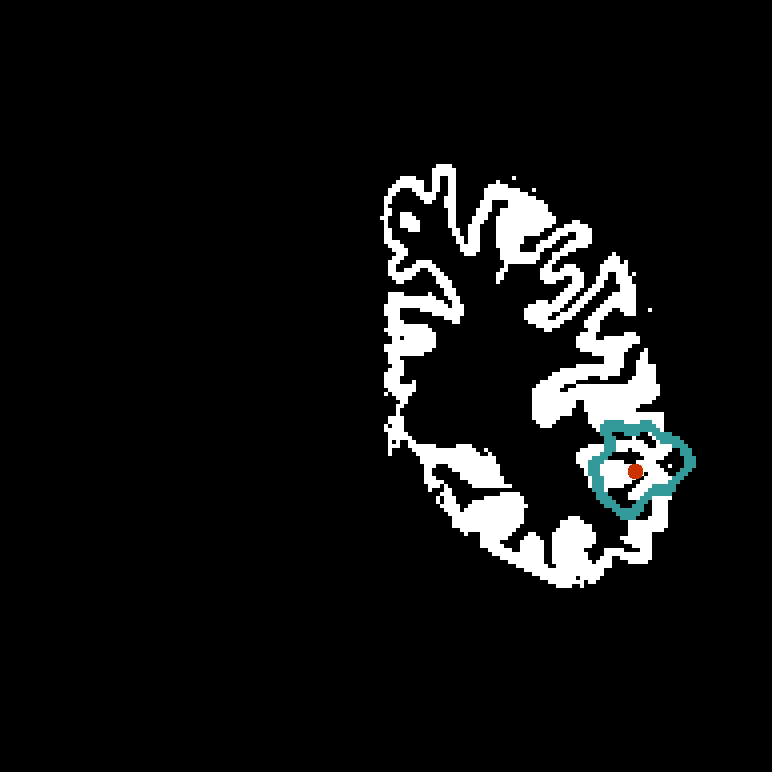
\includegraphics[width=0.8\linewidth]{Ma}
    \caption{$S_a$ on $\M\st{GM}^h$\label{fig:sama}}
  \end{subfigure}
  \begin{subfigure}{0.3\textwidth}
    
\includegraphics[width=0.8\linewidth]{Mb}
    \caption{$S_a$ on $\M\st{R}^h$\label{fig:samb}}
  \end{subfigure}
  \begin{subfigure}{0.3\textwidth}
    
\includegraphics[width=0.8\linewidth]{Mr}
    \caption{$\Y\simul = \M_{S_a} \odot \M\st{R}^h$\label{fig:mr}}
  \end{subfigure}

  \caption[Simulation of the ground-truth cavity label]{
    Simulation of the ground-truth cavity label.
    $S_a$ (blue) is computed by centering $S\st{E}$ on $\bm{a}$, a random positive voxel (red) of $\M\st{GM}^h$ (\subref{fig:sama}).
    $\M_{S_a}$ is a binary mask derived from $S_a$.
    $\Y\simul$ (\subref{fig:mr}) is the intersection of $\M_{S_a}$ and $\M\st{R}^h$ (\subref{fig:samb}).
  }
  \label{fig:shape}
\end{figure}



The simulated \ac{RC} should not span both hemispheres or include extracerebral tissues such as bone or scalp.
This section describes our method to ensure that the \ac{RC} appears in anatomically plausible regions.

A \ac{T1w} \ac{MRI} is defined as $\X\pre : \Omega \to \R$.
A full brain parcellation $\bm{P} : \Omega \to Z$ is generated \cite{cardoso_geodesic_2015} for $\X\pre$,
where $Z$ is the set of segmented structures.
A cortical gray matter mask $\M\st{GM}^h : \Omega \to \{0, 1\}$
of hemisphere $h$ is extracted from $\bm{P}$,
where $h$ is randomly chosen from $H = \{\text{left}, \text{right}\}$ with equal probability.

A ``resectable hemisphere mask'' $\M\st{R}^h$ is generated from $\bm{P}$ and $h$ such that $\M\st{R}^h (\p) = 1$ if
${\bm{P}(\p) \neq \{M\st{BG}, M\st{BT}, M\st{CB}, M_{\hat{h}} \} }$
and $0$ otherwise,
where $M\st{BG}$, $M\st{BT}$, $M\st{CB}$ and $M_{\hat{h}}$ are the labels in $Z$ corresponding to the background, brainstem, cerebellum and contralateral hemisphere, respectively.
$\M\st{R}^h$ is smoothed using a series of binary morphological operations, for realism.


A random voxel $\bm{a} \in \Omega$ is selected such that $\M\st{GM}^h(\bm{a}) = 1$.
A translation transform $T\st{T}(\bm{a} - \bm{c})$ is applied to $S\st{E}$ so $S_a = T\st{T}(\bm{a} - \bm{c}) (S\st{E})$ is centered on $\bm{a}$.

A binary image $\binimg{\M_{S_a}}$ is generated from $S_a$ such that $\M_{S_a}(\p) = 1$ for all $\p$ within $S_a$ and $\M_{S_a}(\p) = 0$ outside.
Finally, $\M_{S_a}$ is restricted by $\M\st{R}^h$ to generate the cavity label $\Y\simul = \M_{S_a} \odot \M\st{R}^h$, where $\odot$ represents the Hadamard product.
\cref{fig:shape} illustrates the process.



\subsubsection{Simulating cavities filled with CSF}
\label{sec:texture_cavity}

Brain \acp{RC} are typically filled with \ac{CSF}.
To generate a realistic \acs{CSF} texture,
we create a ventricle mask
${\M\st{V} : \Omega \to \{ 0, 1 \}}$ from $\bm{P}$, such that
$\M\st{V}(\p) = 1$ for all $\p$ within the ventricles and
$\M\st{V}(\p) = 0$ outside.
Intensity values within the ventricles are assumed to have
a normal distribution \cite{gudbjartsson_rician_1995}
with a mean $\mu\st{CSF}$ and standard deviation $\sigma\st{CSF}$
calculated from voxel intensity values in
$\{ \X\pre(\p) \mid \p \in \Omega \land \M\st{V}(\p) = 1 \}$.
A \acs{CSF}-like image is then generated as $\X\st{CSF}(\p) \sim \NN (\mu\st{CSF}, \sigma\st{CSF}), \forall \p \in \Omega$.


We use $\Y\simul$ to guide blending of $\X\st{CSF}$ and $\X\pre$ as follows.
A Gaussian filter is applied to $\Y\simul$ to obtain a smooth alpha channel $\img{\AAA_\alpha}{[0, 1]}$ defined as
$
  \AAA_\alpha
  = \Y\simul
  * \bm{G}_{\NN}(\bm{\sigma}),
$
where
$*$ is the convolution operator
and $\bm{G}_{\NN}(\bm{\sigma})$ is a 3D Gaussian kernel with standard deviations
$\bm{\sigma} = (\sigma_x, \sigma_y, \sigma_z)$.
Then, $\X\st{CSF}$ and $\X\pre$ are blended by the convex combination
\begin{equation}
  \X\simul
  = \AAA_\alpha \odot \X\st{CSF}
  + (1 - \AAA_\alpha) \odot \X\pre
\end{equation}

We use $\bm{\sigma} > 0$ to mimic partial-volume effects at the cavity boundary.
The blending process is illustrated in \cref{fig:texture}.


\begin{figure}
  \centering
  \captionsetup[subfigure]{aboveskip=3pt, belowskip=5pt}

  \begin{subfigure}{0.15\textwidth}
    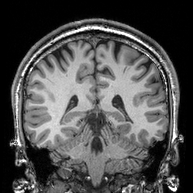
\includegraphics[width=0.99\linewidth]{texture_mri}
    \caption{\label{fig:tmri}}
  \end{subfigure}
  \begin{subfigure}{0.15\textwidth}
    
\includegraphics[width=0.99\linewidth]{texture_checkerboard}
    \caption{\label{fig:checkerboard}}
  \end{subfigure}
  \begin{subfigure}{0.15\textwidth}
    
\includegraphics[width=0.99\linewidth]{Mr}
    \caption{\label{fig:tmh}}
  \end{subfigure}
  \begin{subfigure}{0.15\textwidth}
    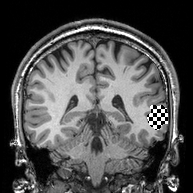
\includegraphics[width=0.99\linewidth]{texture_hard}
    \caption{\label{fig:blh}}
  \end{subfigure}
  \begin{subfigure}{0.15\textwidth}
    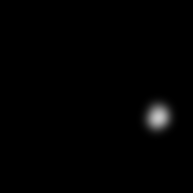
\includegraphics[width=0.99\linewidth]{texture_mask_soft}
    \caption{\label{fig:tms}}
  \end{subfigure}
  \begin{subfigure}{0.15\textwidth}
    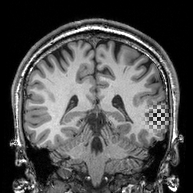
\includegraphics[width=0.99\linewidth]{texture_soft}
    \caption{\label{fig:bls}}
  \end{subfigure}

  \caption[Simulation of resected image using alpha blending]{
    Simulation of resected image $\X\simul$.
    We use a checkerboard for visualization.
    Two scalar-valued images $\X\pre$ (\subref{fig:tmri})
    and $\X_2$ (\subref{fig:checkerboard})
    are blended using $\Y\simul$ (\subref{fig:tmh})
    and $\sigma_i = \SI{0}{\milli \meter}$ to create an image with hard boundaries (\subref{fig:blh})
    and $\sigma_i = \SI{5}{\milli \meter}$ (\subref{fig:tms})
    for an image with soft boundaries (\subref{fig:bls}),
    mimicking partial-volume effects.
  }
  \label{fig:texture}
\end{figure}

% % \input{tex/sections/methods/semisupervised}

\section{Example of clinical usage}

% Pt # 771 (0999, roaj) This patient was a 28-year-old right-handed gentleman assessed for epilepsy surgery having had nocturnal generalised seizures since the age of 12 and subsequently developed stereotyped head and eye version to the right with body turning, tonic left leg extension and raising of the left arm with speech arrest. Ictal EEG was non lateralising and interictal EEG showed bitemporal sharp waves. MRI showed cortical dysplasia in the left superior frontal gyrus and Ictal SPECT highlighted superior more than middle frontal gyrus; intracranial EEG was performed to map eloquent cortex and a left frontal resection including the supplementary motor cortex resulted in complete seizure-freedom for 4 years (ILAE 1 for four years of follow up).

In this section, we demonstrate a usage example of our \ac{SVT} for a retrospective case of a patient who underwent epilepsy resective surgery at the \ac{NHNN} (Queen Square, London, UK).
We use the \texttt{mega\_analysis} querying module, which uses the \svtdatabase database \cite{alim-marvasti_mapping_2021,alim-marvasti_probabilistic_2021}.

The patient was right-handed and presented head version to the right at the beginning of seizures.
Ictal \ac{EEG} was non lateralizing and interictal \ac{EEG} showed bitemporal sharp waves.
We used the patient's preoperative \ac{T1w} \ac{MRI} as reference for the visualization.
The Neuromorphometrics brain parcellation was generated using \ac{GIF} \cite{cardoso_geodesic_2015}.

We queried the database using the semiology \textit{Head version (right)} and setting the dominant hemisphere to \textit{Left}.
The most highlighted structures concentrate in the left frontal lobe (\cref{fig:svt_case_heatmap}).

\begin{figure}[!ht]
  \centering
  \svtscreenshot{svt_case_heatmap}
  \caption[Querying the database using a retrospective real case]{
    Querying the database using data from a retrospective real case.
    The selected semiology term was \textit{Head version (right)}, and the dominant hemisphere was \textit{Left}.
    The regions with highest numbers of datapoints concentrate around the left frontal lobe (represented on the right side of the axial and coronal views).
  }
  \label{fig:svt_case_heatmap}
\end{figure}

As this is a retrospective case from a patient who underwent resective surgery some years ago, the postoperative \ac{MRI} and the clinical outcome are available.
We used a rigid registration algorithm to align the preoperative and postoperative \acp{MRI} for visualization purposes \cite{ourselin_block_2000}.
As non-rigid brain deformations may happen after the surgery and we used a rigid registration, the alignment is only approximate; however, it is accurate enough for a visual analysis.
When visualizing the aligned images, including the probability map, we observed an overlap between the highlighted areas (i.e., the brain structures with the highest number of datapoints) and the resection cavity (\cref{fig:svt_resection}).
The surgery was successful and resulted in complete seizure freedom.

\begin{figure}[!ht]
  \centering
  \svtscreenshot{svt_resection}
  \caption[Comparison of the probability map and the postoperative MRI]{
    Qualitative comparison of the \ac{EZ} probability map and the postoperative \ac{MRI}.
    Note the overlap between the highlighted structures and the resection cavity.
    The images were rigidly registered, and the crosshairs are centered on approximately the same brain region.
    The patient became seizure-free after resective surgery.
  }
  \label{fig:svt_resection}
\end{figure}

\section{Discussion and conclusion}
\label{sec:discussion}

We addressed the challenge of segmenting postoperative brain \acp{rc} from \ac{T1w} \ac{MRI} without annotated data.
We developed a self-supervised learning strategy to train without manually annotated data, and a method to simulate \acp{RC} from preoperative \ac{MRI} to generate training data.
Our novel approach is conceptually simple, easy to implement, and relies on clinical knowledge about postoperative phenomena.
The resection simulation is computationally efficient ($< \SI{1}{\second}$), so it can run during training as part of a data augmentation pipeline.
It is compatible with the TorchIO framework \cite{perez-garcia_torchio_2021} to leverage other data argumentation techniques during training, enabling our model to have a robust performance across \ac{MRI} of variable quality.

Modeling a realistic cavity shape is important (\cref{sec:self}).
Our model generalizes well to clinical data from different institutions and pathologies, including epilepsy and glioma.
Models may be easily fine-tuned using small annotated clinical datasets to improve performance.
Moreover, our resection simulation and learning strategy may be extended to train with arbitrary modalities, or synthetic modalities generated from brain parcellations \cite{billot_learning_2020}.
Therefore, our strategy can be adopted by institutions with a large amount of unlabeled data, while fine-tuning and testing on a smaller labeled dataset.

Poor segmentation performance is often due to very small cavities, where the cavity was not detected, and large brain shift or subdural edema, where regions were incorrectly segmented.
The former issue may be overcome by training with a distribution of cavity volumes which oversamples small resections.
The latter can be addressed by extending our method to simulate displacement with biomechanical models or nonlinear deformations of the brain \cite{granados_generative_2021}.

The baseline model performance improved by leveraging unlabeled postoperative images for semi-supervised learning, but remained lower than inter-rater variability \cite{perez-garcia_simulation_2020}.  % TODO: add this info in this thesis!
We believe that a setting with a smaller training dataset might benefit further from the semi-supervised approach.
However, we did not perform an extensive assessment of our semi-supervised approach as this is out of the scope of this paper.

We showed that our model correctly segmented an intraoperative image, respecting imaginary boundaries between brain and skull, suggesting a good inductive bias of human neuroanatomy.
Qualitative results and execution time, which is in the order of milliseconds, suggest that our method could be used intraoperatively, for image guidance during resection or to improve registration with preoperative images by masking the cost function using the \ac{RC} segmentation \cite{brett_spatial_2001}.
Segmenting the \ac{RC} may also be used to study potential damage to white matter tracts postoperatively \cite{winston_optic_2012}.
Our method could be easily adapted to simulate other lesions for self-supervised training, such as cerebral microbleeds \cite{cuadrado-godia_cerebral_2018}, narrow and snake-shaped \acp{RC} typical of disconnective surgeries \cite{mohamed_temporoparietooccipital_2011}, or \acp{RC} with residual tumor \cite{meier_automatic_2017}.

As part of this work, we curated and released EPISURG, an \ac{MRI} dataset with annotations from three independent raters.
EPISURG could serve as a benchmark dataset for quantitative analysis of pre- and postoperative imaging of open resection for epilepsy treatment.
To the best of our knowledge, this is the first open annotated database of post-resection \ac{MRI} for epilepsy patients.


\onehalfspacing % a blank line seems to be needed before this command
